\documentclass[11pt]{article}

\usepackage{latexsym}
\usepackage{amsmath}
\usepackage{amssymb}
\usepackage{amsthm}
\usepackage{graphicx}
\usepackage{cite}
\usepackage{wrapfig}
\usepackage{pseudocode}
\usepackage{url} 
\usepackage[backref, colorlinks=true, citecolor=red, urlcolor=blue, pdfauthor={Jyh-Ming Lien}]{hyperref}


\newcommand{\handout}[5]{
  \noindent
  \begin{center}
  \framebox{
    \vbox{
      \hbox to 5.78in { {\bf } \hfill #2 }
      \vspace{4mm}
      \hbox to 5.78in { {\Large \hfill #5  \hfill} }
      \vspace{2mm}
      \hbox to 5.78in { {\em #3 \hfill #4} }
    }
  }
  \end{center}
  \vspace*{4mm}
}

\newcommand{\lecture}[4]{\handout{#1}{#2}{#3}{#4}{#1}}

\newtheorem{theorem}{Theorem}
\newtheorem{corollary}[theorem]{Corollary}
\newtheorem{lemma}[theorem]{Lemma}
\newtheorem{observation}[theorem]{Observation}
\newtheorem{proposition}[theorem]{Proposition}
\newtheorem{definition}[theorem]{Definition}
\newtheorem{claim}[theorem]{Claim}
\newtheorem{fact}[theorem]{Fact}
\newtheorem{assumption}[theorem]{Assumption}

% 1-inch margins, from fullpage.sty by H.Partl, Version 2, Dec. 15, 1988.
\topmargin 0pt
\advance \topmargin by -\headheight
\advance \topmargin by -\headsep
\textheight 8.9in
\oddsidemargin 0pt
\evensidemargin \oddsidemargin
\marginparwidth 0.5in
\textwidth 6.5in

\parindent 0in
\parskip 1.5ex
%\renewcommand{\baselinestretch}{1.25}

\begin{document}

\lecture{Assignment Report}{Fall 2017}{Jixuan Zhi}{Advance Algorithm Programming}

\section{Summary of the two methods}

\subsection{hedcuter method}
\subsubsection{Voronoi diagram}
The hedcut use the image-based wave propagation method\cite{secord2002weighted}.
\\\\Firstly, create n(1000) points in the image, the more black area has higher probabily.
Define a density function $p(x,y)=1-f(x,y)$,where $0\leq\;f(x,y)\leq\;1$ is the range from
a black pixel to a white pixel. Calculate every site's density that we randomly created from
the definition. In the distance image, initial every pixel's distance to $+\infty\;$except the 
sites, each site is given a unique ID. Storing every site in a heap, for every site, check its 8 neighbors,
update its distance by minimum the distance of its original distance and sum of its density with site's distance, if the distance updated, update the ID as the same as site and put the pixel in the heap. Now we have more pixels in the pixel, check them one by one from the least distance, repeated the updated process until the heap is empty. 
\\\\Now we have a voronoi diagram, because every pixel has an ID which means it belongs to the unique site.
\subsubsection{Centroidal Voronoi tessellation(CVT)}
For a centroidal voronoi diagram, using an iterative algorithm\cite{secord2002weighted} to generate it. For a voronoi diagram generated by n points, compute the centroid of each cell, move the site to its centroid, calculate the voronoi diagram again, repeated the process until the point is already its centroid. In practice, set an iterative limit number, or set a minimum displacement distance,
calculate displacement distance of each process until it no greater than the minimum one. 
\\\\The method of calculating voronoi diagram we have already talked. For each cell, it has many pixels which have the same ID, calculate the average density and position of the pixels, this is the centroid of the cell.
\subsubsection{Stippling method}
For an image which already has a centroidal vornonoi diagram, the position of each centroid is the position of each stippling point, compute the average intensity of each cell as the intensity of each stippling point. We can also control the radius of each point by its intensity or uniform.

\subsection{voronoi method}
\subsubsection{Voronoi diagram}
The voronoi code use the Fortune's algorithm\cite{fortune1987sweepline}, from the paper "A sweepline algorithm for Voronoi Diagrams" by Steven Fortune. The idea is making transformation on Voronoi diagram, because the lowest point of the transformed Voronoi region of a site appears at the site itself.
\\\\The central part of the algorithm is the Transformation. The mapping $^*$ : $R^2\to\;R^2$ defined by $^*(x,y)=(x,y+d(x,y))$, where $d(x,y)$ is a radius of a voronoi circle centered at $(x,y)$, and $(x,y)$ is usually in the voronoi edge. From the transformation, a bisector is changed to a hyperbola or a vertical half line, and for the voronoi region of each site, map function maps all the points below the site to points above the site or the site itself. The site is the lowest point of the region. The transformation is one to one relationship. 
\\\\Now we can use the plane sweep algorithm, moves a horizontal line upwards across the plane maintaining the regions of $V^*$ intersected by the horizontal line. The bisector is changed to a hyperbola than opens upwards, and we can define them as two parts: left and right, meaning for the position of the site. The input is n points, the output is each site with a list of bisectors.
\\\\For the data structures, in the codes, maintaining two priority queues, one for each site, one for vertices created by the intersection of edges. Every time we choose the lowest point of this two queues.
Also maintaining a sequence of boundaries L in the order from left to right. Use the half edge here.
\\\\There are two events, site event and vector event which the point is the intersection of edges.
\\\\For site event p, find the a region $R_q^*$ on L containing p, create bisector $B_pq^*$. Update list L
so that it contains left edge, $R_P^*$, right edge. Insert intersections between left and right edge with
neighboring boundaries in the queue of the intersection.
\\\\For vector event, let p be the intersection of boundaries $E_qr$ and $E_rs$. Create the bisector $B_qs^*$.
Update list L so it contains $E_qs$, left or right edge, instead of $E_qr$, $R_r^*$,$E_rs$.Delete from the intersection queue between $E_qr$ and its neighbor to the left and between $E_rs$ and its neighbor to the right. Insert any intersections between $E_qs$ and its neighbors to the left or right into intersection queue.
Mark p as a vertex, and as an endpoint of $E_qr$, $E_rs$, and $E_qs$.
\\\\ Algorithm ends when the two queues are both empty.


\subsubsection{Centroida Voronoi tessellation(CVT)}
For a centroidal voronoi diagram, still using the iterative algorithm\cite{secord2002weighted} we talked before.
compute the centroid of each cell in the voronoi diagram, move the site to its centroid, calculate the voronoi diagram again, repeated the process until the site is already its centroid. In practice, set a minimum displacement distance, calculate displacement distance of each process until it no greater than the minimum one. 
\\To calculate the centroid of each cell, each site has an edge list which is the boundary of the cell. For the pixels in this cell, calculate
the average density and position of the pixels, that is the centroid of the cell.

\subsubsection{Stippling method}
The method is similar to the method of hedcut. For an image which already has a centroidal voronoi diagram, the position of each centroid is the position of each stippling point, the radius of each point is defined by the distance between the centroid and the closest point or farthest point. The intensity of the point is black or color.

\section{Comparison of the two methods}

\subsection{Test results}
I tested the two different methods using different images. To compare the results, I set the all the parameters to be equal, such as the same subpixels. 
\\\\I used different stipple points(1000, 4000, 16000) to test the same image. Figure 1,3,5 which use the hedcut method, Firgure 2,4,6 which use the voronoi method. The red circles give some differences between two methods.


\begin{figure}[htbp]
\centering
\begin{minipage}[t]{0.48\textwidth}
\centering
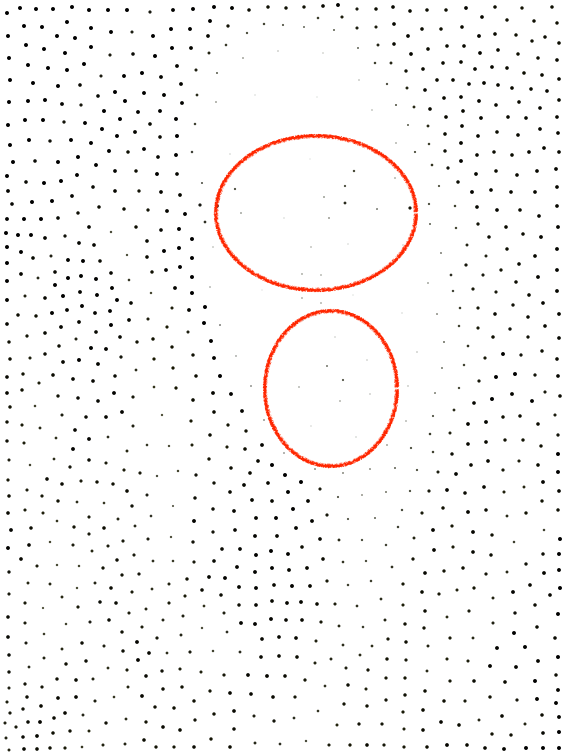
\includegraphics[width = 0.9\textwidth]{fairyeyes-1000.png}
\caption{1000 stipple points}
\end{minipage}
\begin{minipage}[t]{0.48\textwidth}
\centering
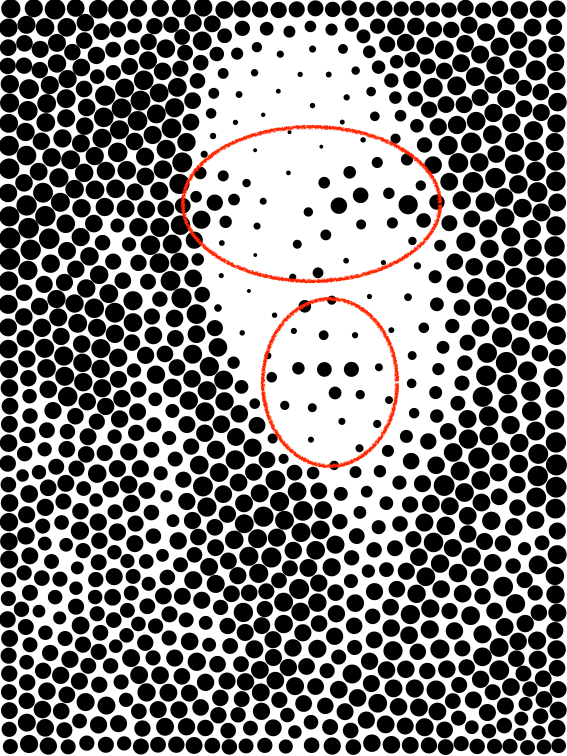
\includegraphics[width = 0.9\textwidth]{faireyes_vor_1000.png}
\caption{1000 stipple points}
\end{minipage}
\end{figure}


\begin{figure}[htbp]
\begin{minipage}[t]{0.48\textwidth}
\centering
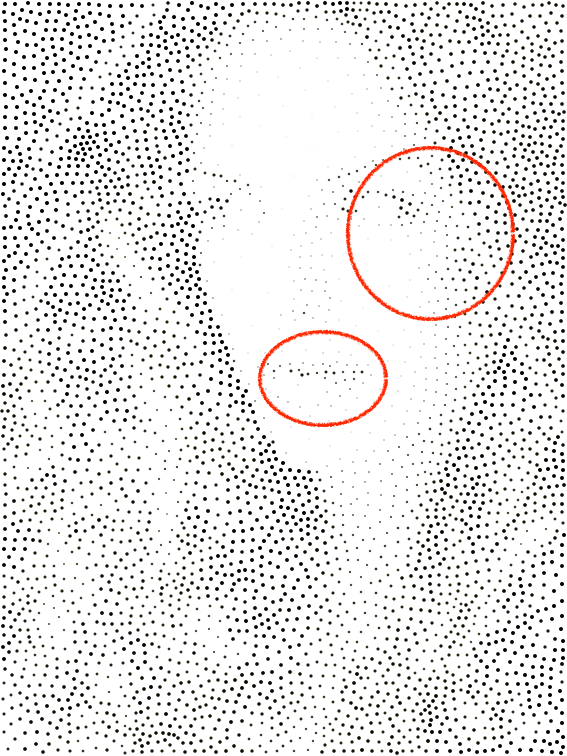
\includegraphics[width = 0.9\textwidth]{fairyeyes-4000.png}
\caption{4000 stipple points}
\end{minipage}
\begin{minipage}[t]{0.48\textwidth}
\centering
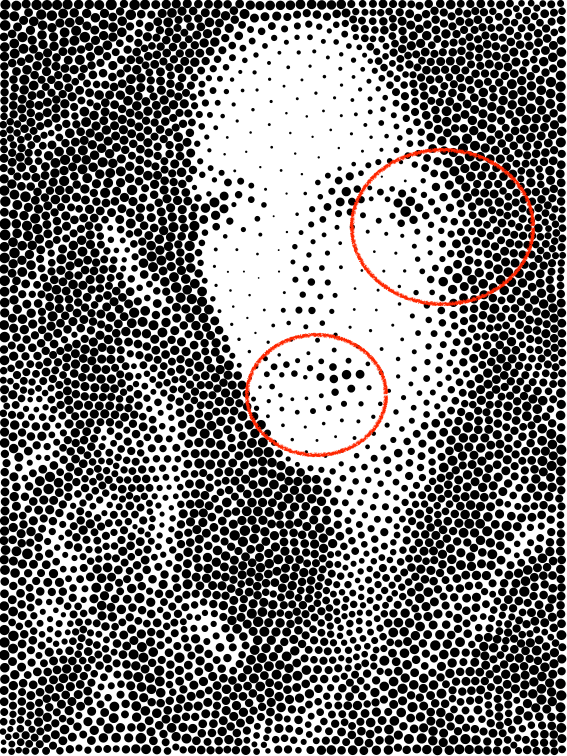
\includegraphics[width = 0.9\textwidth]{faireyes_vor_4000.png}
\caption{4000 stipple points}
\end{minipage}
\end{figure}

\begin{figure}[htbp]
\centering
\begin{minipage}[t]{0.48\textwidth}
\centering
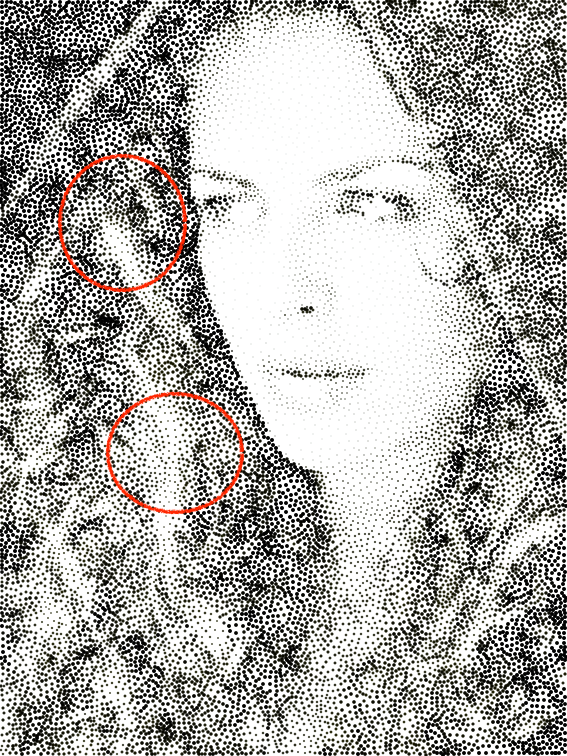
\includegraphics[width = 0.9\textwidth]{fairyeyes-16000.png}
\caption{16000 stipple points}
\end{minipage}
\begin{minipage}[t]{0.48\textwidth}
\centering
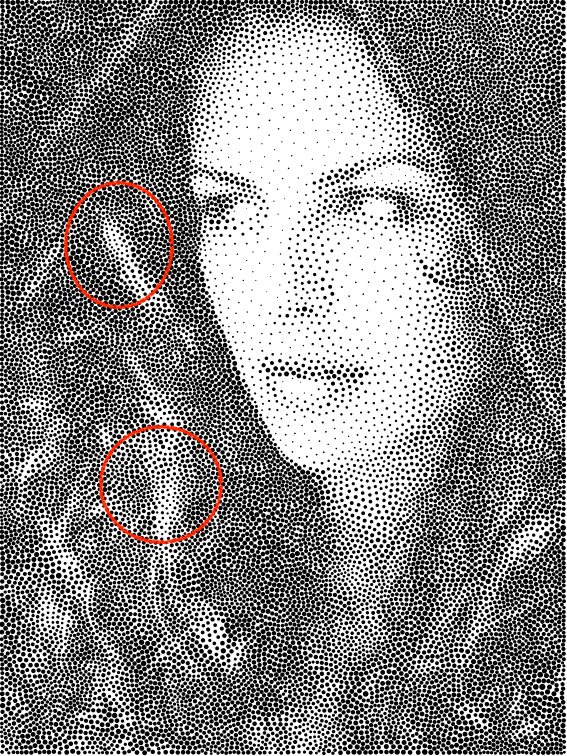
\includegraphics[width = 0.9\textwidth]{f_vor_16000.png}
\caption{16000 stipple points}
\end{minipage}
\end{figure}



From the 6 images, we can have some facts.
\begin{enumerate}
\item voronoi method has a larger size of disc output than the hedcut method disc output, from the figure 1 and figure 2, we can see clearly.
\item In a small number of points such as 1000, see figure 1 and figure 2, it is hard to find the shape of facial features by hedcut method, but voronoi method has some large points to display the facial features.
\item In a median number of points such as 4000, see figure 3 and figure 4, both methods have the shape of facial feature, and the hedcut method has a more natural output, the voronoi method seems not natural.
\item In a large number of points such as 16000, see figure 5 and figure 6, both methods have more clearly shape of the input image shape. But the voronoi method has better well-spaced points than the hedcut method, especially in the area of hair.

\end{enumerate}



\subsection{Some discusstions}
\begin{enumerate}
\item Do you get the same results by running the same program on the same image multiple times? 
\\\\No, because the initial points are different each time, and also the computation has errors, the results are different. 

\item If you vary the number of the disks in the output images,  do these implementations produce the same distribution in the final image? If not, why?
\\\\No, because of the initial points position and calculation errors, resulst are different. And we can observe some facts: If the number of the disks is small, the output images are different which can be observed by naked eyes, if the number of disks is large, the output images are similar, the differences can be got by data. 

\item If you vary the number of the disks in the output images,  is a method faster than the other? 
\\\\Yes, the voronoi method is much faster than the hedcut method, because voronoi method only address the site event and intersection event, about $o(n)$ events, but the hedcut method need address all the pixels in the image, not just $n$ initial points, the number may be much larger than $n$. 

\item Does the size (number of pixels), image brightness or contrast of image increase or decrease their difference? 
\\\\With the size increase, the differences between two methods decreased because their voronoi diagram is much similar. 
\\ Image brightness and contrast may affect the difference between tho methods. With large brightness, the differences decreased because the white area increased and both the face features disappeared, and with less brightness, the face features are clear because we have more black points, so it also decreases the differences. The contrast is the similar thing. 


\item Does the type of image (human vs. machine,  natural vs. urban landscapes, photo vs. painting, etc) increase or decrease their difference? 
\\\\The type of image has no effects on the differences of the method with my experiments. The most important thing is the quality of input image.  

\item Are the outputs of these stippling methods different the hedcut images created by artists (e.g. those from the \href{http://www.wsj.com/articles/SB10001424052748704207504575129961786135180}{Wall Street Journal})? 
\\\\Yes, they are different. We know well-spaced is a feature of a good stipple drawing, the artists achieve this by hand. They need to know the quality of object, image and light. The output is good but defined by artists. But the computists address this by Centroida Voronoi diagram, which has already included all the information it needed.


\end{enumerate}








\section{Improvement of hedcuter method}
\subsection{Sampling strategy based on dithering}
The original sampling is a simple rejection method, I observed that the method still put some points in the
white area, which took so much time to move the site from the white area to black area. So I decided to use Floyd-Steinbery dithering method\cite{floydSteinberg1976dithering} to transform the gray image of the input image to black-and-white image. In the transformed image, just initializes the points to a black pixel in uniform distribution and rejects the white pixel.
\\\\In experiments, I used two different sampling methods with the same number of stipple points. From the figure 7 and figure 8, we could see the dithering method is better than the original method because it rejected the white area. 


\begin{figure}[htbp]
\centering
\begin{minipage}[t]{0.48\textwidth}
\centering
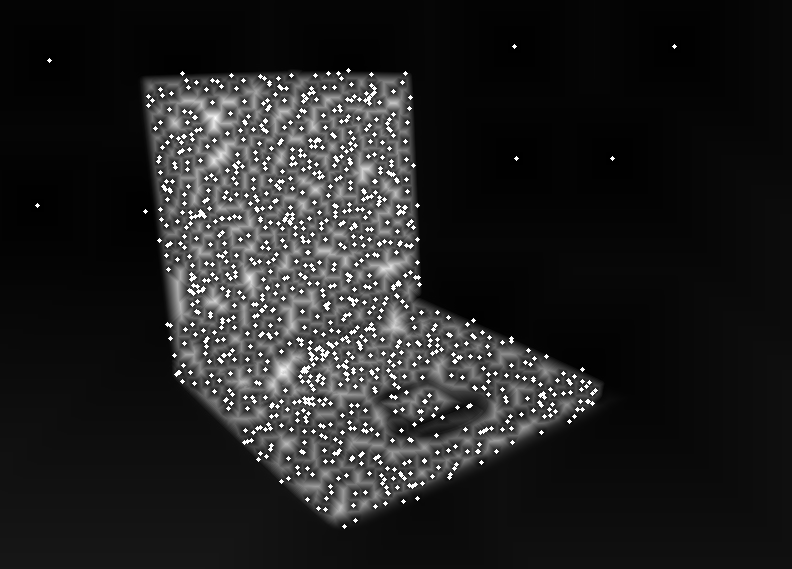
\includegraphics[width = 0.9\textwidth]{new_sam.png}
\caption{dithering sampling}
\end{minipage}
\begin{minipage}[t]{0.48\textwidth}
\centering
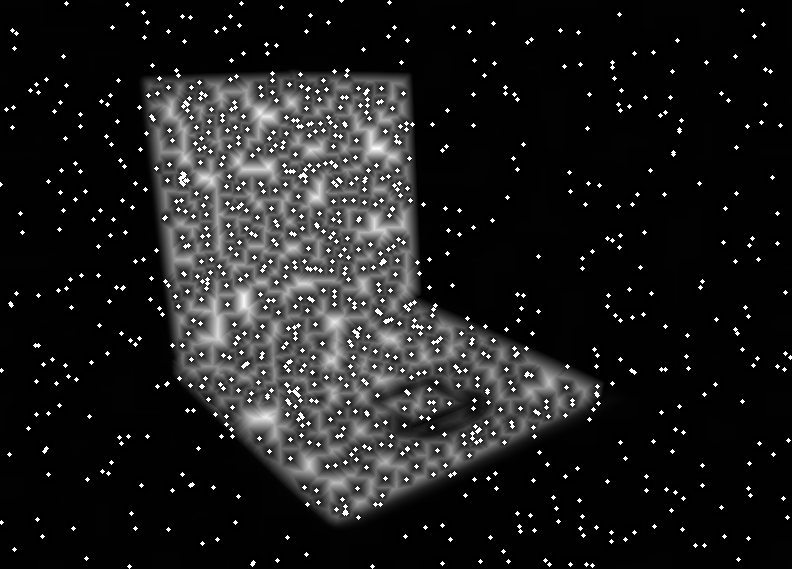
\includegraphics[width = 0.9\textwidth]{old_sam.png}
\caption{original sampling}
\end{minipage}
\end{figure}




\subsection{Disc size based on size and intensity of voronoi cell}
The original disc size is a constant or the largest disc size is a constant. I observed that sometimes the disc is too small to observe or too large to overlap. It is difficult for users to decide a proper disc size.
\\\\ From the voronoi method, I got the idea to draw the disc with the size and intensity of the voronoi cell.
If only using the size, the voronoi in the shallow area is large and caused the disc is so large, the stippling is bad here, so the point size should equal to size of the cell times intensity of the cell.
\\\\To compute the size of voronoi cell, we need to know the boundaries of the cell. The brute-force approach simply examines each pair of adjacent cells. If the ID of cells are different, the location is registered as a point on a Voronoi. For every cell, check the distance between the site and its boundary point, decide the closest distance as the size of the cell. The cell's intensity is similar to calculate the centroid, compute the sum of every pixels' intensity in the cell, divided by the sum of max intensity. 
\\\\To test the results, I added a command "-vorsize" to specify the method. I test the new method comparing to the original method with the same input image, see figure 9 and figure 10. The new method has larger and clearer point, so it showed more information about the input image. I sampled different numbers of points to the same image. The result of larger number of points is better than the small number, see figure 11 and figure 12. Compare figure 11 with figure 1, the face features are more clear. 
   
\begin{figure}[htbp]
\centering
\begin{minipage}[t]{0.48\textwidth}
\centering
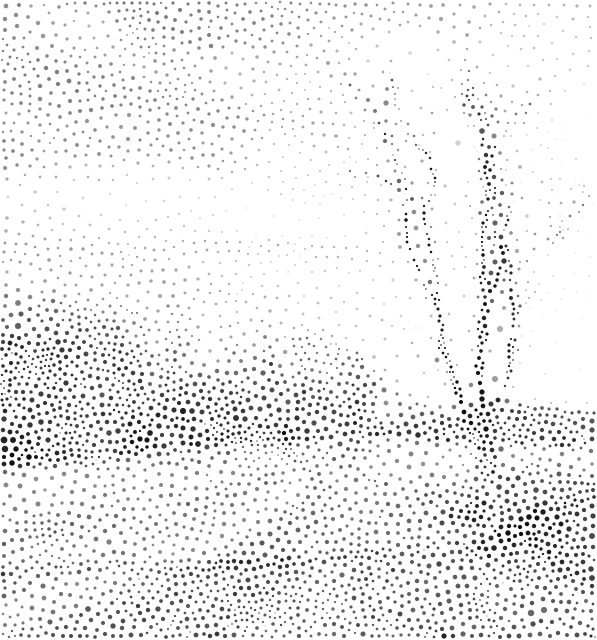
\includegraphics[width = 0.9\textwidth]{new_nature-4000.png}
\caption{new disc size}
\end{minipage}
\begin{minipage}[t]{0.48\textwidth}
\centering
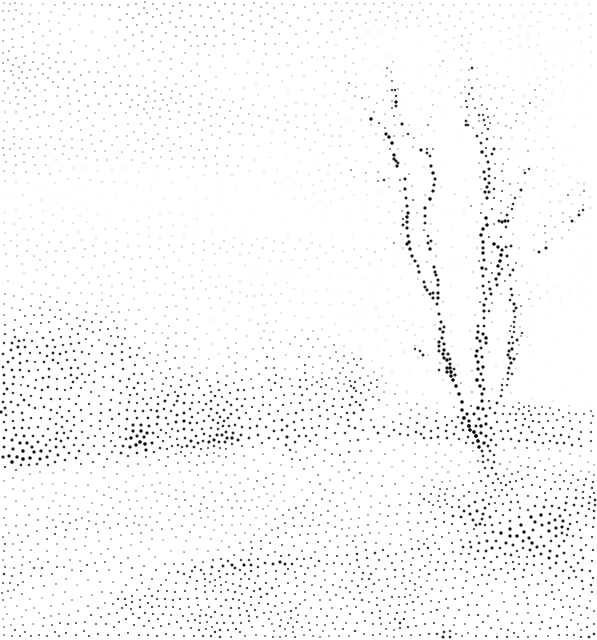
\includegraphics[width = 0.9\textwidth]{old_nature-4000.png}
\caption{old disc size}
\end{minipage}
\end{figure}

\begin{figure}[htbp]
\centering
\begin{minipage}[t]{0.48\textwidth}
\centering
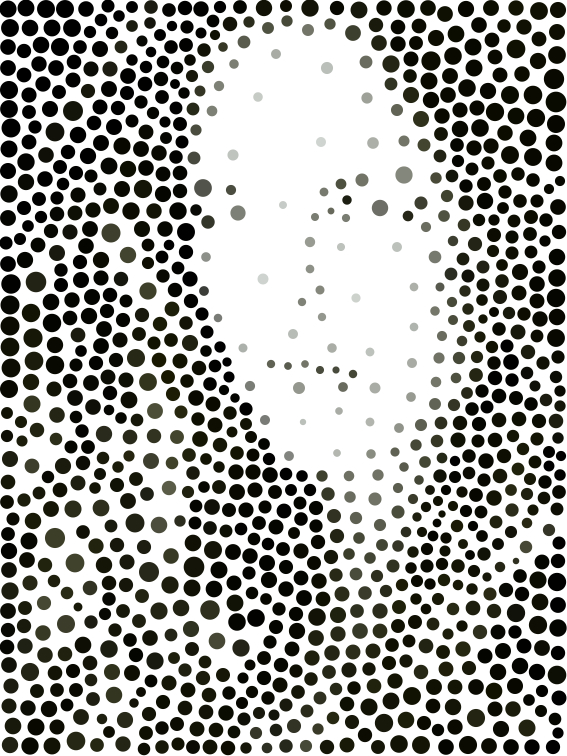
\includegraphics[width = 0.9\textwidth]{f-1000-new.png}
\caption{new disc size with 1000 points}
\end{minipage}
\begin{minipage}[t]{0.48\textwidth}
\centering
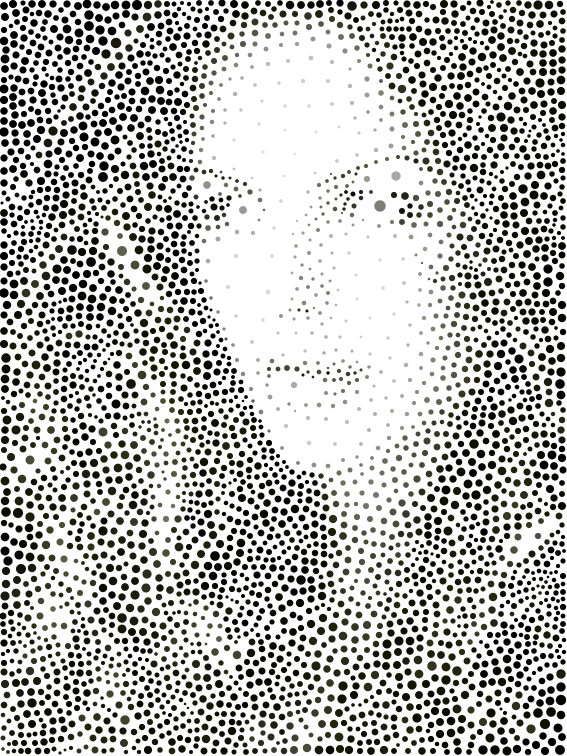
\includegraphics[width = 0.9\textwidth]{f-4000-new.png}
\caption{new disc size with 4000 points}
\end{minipage}
\end{figure}





\subsection{GPU method}
The hedcut code only has a start implementation of GPU method. I decided to make a progress. The idea is simple, the algorithm\cite{hoff1999fast} draws a set of cones with their apexes at each point. The cones all have the same height and base, we view the cones from the above the cones with an orthogonal projection. In addition, each cone has a unique color, the depth-buffer decides for each pixel with the proper color. We can scan the resulting image and determine each pixel's belonging to by its unique colors, and then we got voronoi diagram.
\\\\To make unique color, we use RGB values to encode, each value has $2^8$ bit, but we only use red and green value, having $2^16 = 65536$ different possibilities and we assigned the blue value as the same as red value, with unicoding the value, we can get the unique ID and know the pixel's belonging. To calculate the centroid, the method is similar as we talked, and we can repeat the procedure to get better centroidal voronoi diagram.
\\\\The method has some drawbacks. first, the number of generators decremented after each procedure if I removed the empty cells, to keep the number consistent, I decided to keep the point of empty cell to attend next procedure. Second, the largest move displacement which decides the end of the loop is usually larger because some generator cell is empty. It's hard to use the displacement to end the loop. Lastly and maybe the most importantly, we can not get out of GPU computation and stipple the image, because the OpenGL Utility Toolkit(glut) is too old and does not provide the mechanism to get out and resume another code. So I may try another library such GLFW to initialize the openGL in the future.
\\\\Here are some figures to illustrate the GPU method. See figure 13 and figure 14, figure 13 shows the initial state of voronoi diagram based on GPU, figure 14 shows the end state of voronoi diagram after 100 loops. It seems has some effect but still need to figure out in the future.

\begin{figure}[htbp]
\centering
\begin{minipage}[t]{0.48\textwidth}
\centering
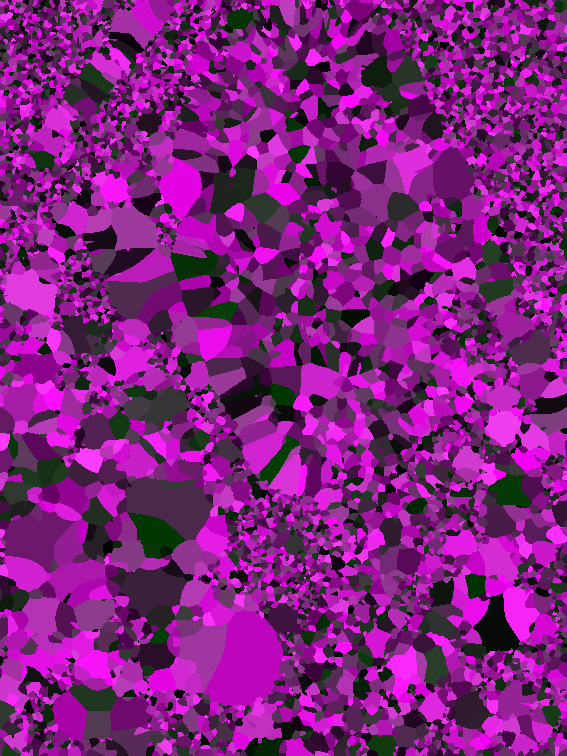
\includegraphics[width = 0.9\textwidth]{gpu_start.png}
\caption{start state}
\end{minipage}
\begin{minipage}[t]{0.48\textwidth}
\centering
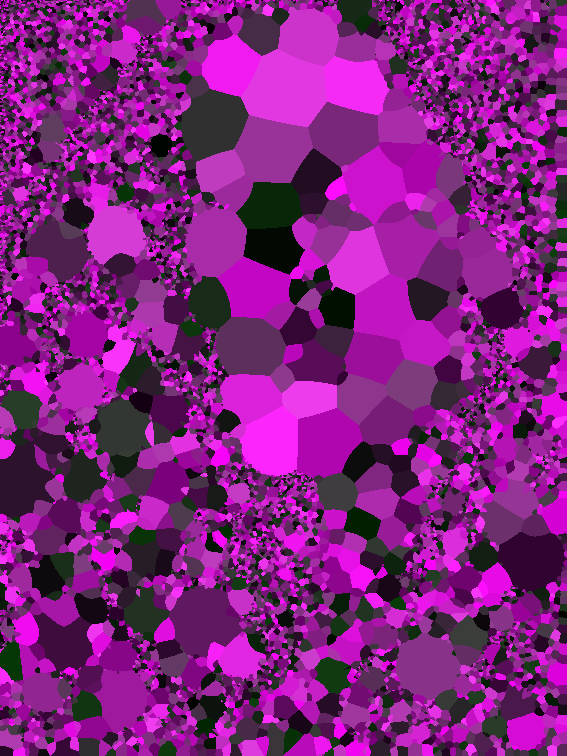
\includegraphics[width = 0.9\textwidth]{gpu_end.png}
\caption{end state}
\end{minipage}
\end{figure}






\bibliographystyle{plain}
\bibliography{report}



\end{document}


